\documentclass {article}
\usepackage {geometry}
\usepackage {CJK}
\usepackage {amsmath}
\usepackage {amssymb}
\usepackage {indentfirst}
\usepackage {listings}
\usepackage {graphicx}

\lstset{basicstyle=\ttfamily,breaklines=true,numbers=left}

\begin{document}
  \begin {CJK*} {UTF8} {gbsn}
		\title {\textbf {\Huge Homework 8 \& Homework 9}}
		\author {郭天魁 \\ 信息科学技术学院 \\ 1300012790}

		\maketitle

		\section{Homework 8}
			\subsection{4.51}
				若在EMW三个阶段中将要对当前的d\_srcA,d\_srcB进行写入,即发生了数据冒险,则将FD暂停,并在E处插入bubble。\\

				需要注意:
				\begin{enumerate}
					\item 在D阶段中,如果是错误预测分支,那么应该插入bubble而非暂停。
					\item 为正确处理conditional move,应用e\_dstE。
				\end{enumerate}

				具体代码见附录\ref{appendixA}或见附件。\\

			\subsection{4.55}
				错误预测仅可能在icode为IJXX且ifun不为UNCOND(即题中的J\_YES)时发生,将要跳转到的位置应从valC与valP中选择。valP通过valA传递,我们将valC通过valE(在ALU中valE=valC+0)传递。\\

				没什么需要注意的地方,把所有错误预测分支的情况加上对valP和valC(valA和valE)的大小判断,并判断ifun是否为UNCOND即可。在计算PC时,如果是错误预测分支,那么应该选择M\_valE和M\_valA中较大的那个,因为预测的是较小的那个。\\

				具体代码见附录\ref{appendixB}或见附件。\\
				
		\section{Homework 9}
			\subsection{5.15}
				A. 不得不说用ppt画图是我这辈子做过的最蠢的事情了……
				
				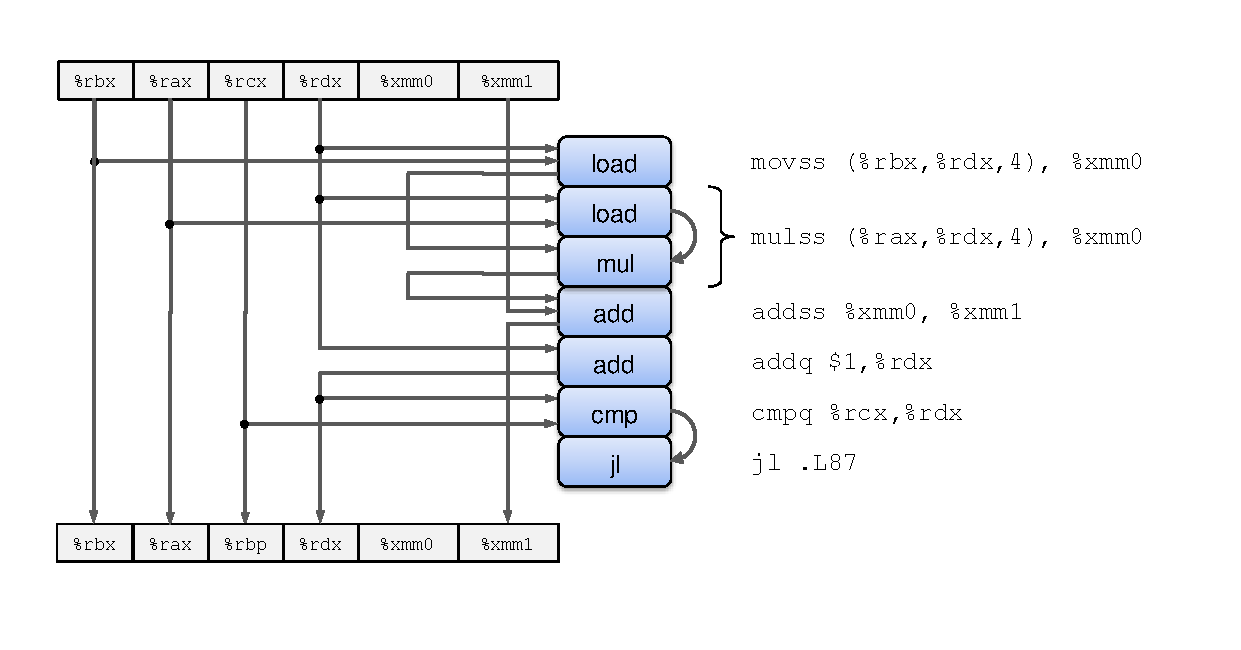
\includegraphics[width=\textwidth]{fpb2a-sequential.pdf}
				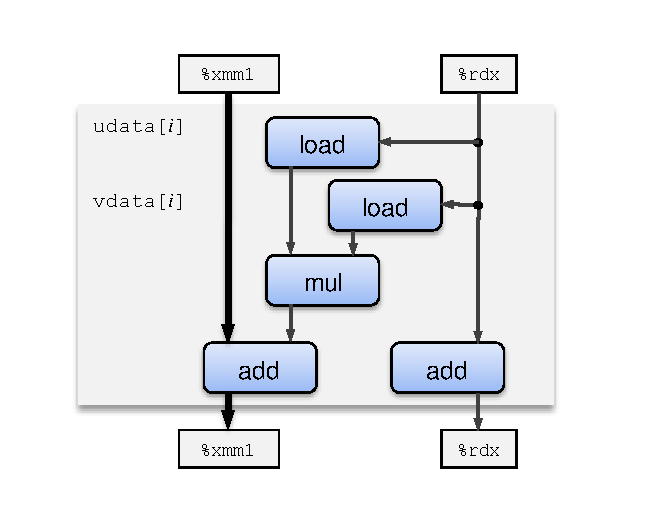
\includegraphics{fpb2a-flow-abstract.pdf}
				
				加粗的即为关键路径。\\
				
				B. 关键路径决定的CPE下界为float加法的延迟3.0。\\
				
				C. 关键路径决定的CPE下界为int加法的延迟1.0。\\
				
				D. 关键路径决定的CPE下界为浮点数加法的延迟3.0。对于需要更多延迟的浮点数乘法,由于其不在循环存储器的数据相关链中,不需要等待前一次迭代的累积值就可以执行,从而消除了瓶颈。\\
				
			\subsection{5.21}
				\begin{lstlisting}[language=C]
void psum2(float a[], float p[], long int n)
{
	long int i;
	float last_val, val;
	last_val = p[0] = a[0];
	for (i = 1; i < n - 1; i += 2) {
		p[i] = last_val + a[i];
		val = a[i] + a[i + 1];
		val = last_val + val;
		p[i + 1] = val;
		last_val = val;
	}
	while(i < n) {
		val = last_val + a[i];
		p[i] = val;
		last_val = val;
	}
}
				\end{lstlisting}
				
			

		\newpage
		\appendix
		\section{pipe-nobypass.hcl}\label{appendixA}
			\begin{lstlisting}
#/* $begin pipe-all-hcl */
####################################################################
#    HCL Description of Control for Pipelined Y86 Processor        #
#    Copyright (C) Randal E. Bryant, David R. O'Hallaron, 2010     #
####################################################################

## Your task is to make the pipeline work without using any forwarding
## The normal bypassing logic in the file is disabled.
## You can only change the pipeline control logic at the end of this file.
## The trick is to make the pipeline stall whenever there is a data hazard.

####################################################################
#    C Include's.  Don't alter these                               #
####################################################################

quote '#include <stdio.h>'
quote '#include "isa.h"'
quote '#include "pipeline.h"'
quote '#include "stages.h"'
quote '#include "sim.h"'
quote 'int sim_main(int argc, char *argv[]);'
quote 'int main(int argc, char *argv[]){return sim_main(argc,argv);}'

####################################################################
#    Declarations.  Do not change/remove/delete any of these       #
####################################################################

##### Symbolic representation of Y86 Instruction Codes #############
intsig INOP 	'I_NOP'
intsig IHALT	'I_HALT'
intsig IRRMOVL	'I_RRMOVL'
intsig IIRMOVL	'I_IRMOVL'
intsig IRMMOVL	'I_RMMOVL'
intsig IMRMOVL	'I_MRMOVL'
intsig IOPL	'I_ALU'
intsig IJXX	'I_JMP'
intsig ICALL	'I_CALL'
intsig IRET	'I_RET'
intsig IPUSHL	'I_PUSHL'
intsig IPOPL	'I_POPL'

##### Symbolic represenations of Y86 function codes            #####
intsig FNONE    'F_NONE'        # Default function code

##### Symbolic representation of Y86 Registers referenced      #####
intsig RESP     'REG_ESP'    	     # Stack Pointer
intsig RNONE    'REG_NONE'   	     # Special value indicating "no register"

##### ALU Functions referenced explicitly ##########################
intsig ALUADD	'A_ADD'		     # ALU should add its arguments

##### Possible instruction status values                       #####
intsig SBUB	'STAT_BUB'	# Bubble in stage
intsig SAOK	'STAT_AOK'	# Normal execution
intsig SADR	'STAT_ADR'	# Invalid memory address
intsig SINS	'STAT_INS'	# Invalid instruction
intsig SHLT	'STAT_HLT'	# Halt instruction encountered

##### Signals that can be referenced by control logic ##############

##### Pipeline Register F ##########################################

intsig F_predPC 'pc_curr->pc'	     # Predicted value of PC

##### Intermediate Values in Fetch Stage ###########################

intsig imem_icode  'imem_icode'      # icode field from instruction memory
intsig imem_ifun   'imem_ifun'       # ifun  field from instruction memory
intsig f_icode	'if_id_next->icode'  # (Possibly modified) instruction code
intsig f_ifun	'if_id_next->ifun'   # Fetched instruction function
intsig f_valC	'if_id_next->valc'   # Constant data of fetched instruction
intsig f_valP	'if_id_next->valp'   # Address of following instruction
boolsig imem_error 'imem_error'	     # Error signal from instruction memory
boolsig instr_valid 'instr_valid'    # Is fetched instruction valid?

##### Pipeline Register D ##########################################
intsig D_icode 'if_id_curr->icode'   # Instruction code
intsig D_rA 'if_id_curr->ra'	     # rA field from instruction
intsig D_rB 'if_id_curr->rb'	     # rB field from instruction
intsig D_valP 'if_id_curr->valp'     # Incremented PC

##### Intermediate Values in Decode Stage  #########################

intsig d_srcA	 'id_ex_next->srca'  # srcA from decoded instruction
intsig d_srcB	 'id_ex_next->srcb'  # srcB from decoded instruction
intsig d_rvalA 'd_regvala'	     # valA read from register file
intsig d_rvalB 'd_regvalb'	     # valB read from register file

##### Pipeline Register E ##########################################
intsig E_icode 'id_ex_curr->icode'   # Instruction code
intsig E_ifun  'id_ex_curr->ifun'    # Instruction function
intsig E_valC  'id_ex_curr->valc'    # Constant data
intsig E_srcA  'id_ex_curr->srca'    # Source A register ID
intsig E_valA  'id_ex_curr->vala'    # Source A value
intsig E_srcB  'id_ex_curr->srcb'    # Source B register ID
intsig E_valB  'id_ex_curr->valb'    # Source B value
intsig E_dstE 'id_ex_curr->deste'    # Destination E register ID
intsig E_dstM 'id_ex_curr->destm'    # Destination M register ID

##### Intermediate Values in Execute Stage #########################
intsig e_valE 'ex_mem_next->vale'	# valE generated by ALU
boolsig e_Cnd 'ex_mem_next->takebranch' # Does condition hold?
intsig e_dstE 'ex_mem_next->deste'      # dstE (possibly modified to be RNONE)

##### Pipeline Register M                  #########################
intsig M_stat 'ex_mem_curr->status'     # Instruction status
intsig M_icode 'ex_mem_curr->icode'	# Instruction code
intsig M_ifun  'ex_mem_curr->ifun'	# Instruction function
intsig M_valA  'ex_mem_curr->vala'      # Source A value
intsig M_dstE 'ex_mem_curr->deste'	# Destination E register ID
intsig M_valE  'ex_mem_curr->vale'      # ALU E value
intsig M_dstM 'ex_mem_curr->destm'	# Destination M register ID
boolsig M_Cnd 'ex_mem_curr->takebranch'	# Condition flag
boolsig dmem_error 'dmem_error'	        # Error signal from instruction memory

##### Intermediate Values in Memory Stage ##########################
intsig m_valM 'mem_wb_next->valm'	# valM generated by memory
intsig m_stat 'mem_wb_next->status'	# stat (possibly modified to be SADR)

##### Pipeline Register W ##########################################
intsig W_stat 'mem_wb_curr->status'     # Instruction status
intsig W_icode 'mem_wb_curr->icode'	# Instruction code
intsig W_dstE 'mem_wb_curr->deste'	# Destination E register ID
intsig W_valE  'mem_wb_curr->vale'      # ALU E value
intsig W_dstM 'mem_wb_curr->destm'	# Destination M register ID
intsig W_valM  'mem_wb_curr->valm'	# Memory M value

####################################################################
#    Control Signal Definitions.                                   #
####################################################################

################ Fetch Stage     ###################################

## What address should instruction be fetched at
int f_pc = [
	# Mispredicted branch.  Fetch at incremented PC
	M_icode == IJXX && !M_Cnd : M_valA;
	# Completion of RET instruction.
	W_icode == IRET : W_valM;
	# Default: Use predicted value of PC
	1 : F_predPC;
];

## Determine icode of fetched instruction
int f_icode = [
	imem_error : INOP;
	1: imem_icode;
];

# Determine ifun
int f_ifun = [
	imem_error : FNONE;
	1: imem_ifun;
];

# Is instruction valid?
bool instr_valid = f_icode in 
	{ INOP, IHALT, IRRMOVL, IIRMOVL, IRMMOVL, IMRMOVL,
	  IOPL, IJXX, ICALL, IRET, IPUSHL, IPOPL };

# Determine status code for fetched instruction
int f_stat = [
	imem_error: SADR;
	!instr_valid : SINS;
	f_icode == IHALT : SHLT;
	1 : SAOK;
];

# Does fetched instruction require a regid byte?
bool need_regids =
	f_icode in { IRRMOVL, IOPL, IPUSHL, IPOPL, 
		     IIRMOVL, IRMMOVL, IMRMOVL };

# Does fetched instruction require a constant word?
bool need_valC =
	f_icode in { IIRMOVL, IRMMOVL, IMRMOVL, IJXX, ICALL };

# Predict next value of PC
int f_predPC = [
	f_icode in { IJXX, ICALL } : f_valC;
	1 : f_valP;
];

################ Decode Stage ######################################


## What register should be used as the A source?
int d_srcA = [
	D_icode in { IRRMOVL, IRMMOVL, IOPL, IPUSHL  } : D_rA;
	D_icode in { IPOPL, IRET } : RESP;
	1 : RNONE; # Don't need register
];

## What register should be used as the B source?
int d_srcB = [
	D_icode in { IOPL, IRMMOVL, IMRMOVL  } : D_rB;
	D_icode in { IPUSHL, IPOPL, ICALL, IRET } : RESP;
	1 : RNONE;  # Don't need register
];

## What register should be used as the E destination?
int d_dstE = [
	D_icode in { IRRMOVL, IIRMOVL, IOPL} : D_rB;
	D_icode in { IPUSHL, IPOPL, ICALL, IRET } : RESP;
	1 : RNONE;  # Don't write any register
];

## What register should be used as the M destination?
int d_dstM = [
	D_icode in { IMRMOVL, IPOPL } : D_rA;
	1 : RNONE;  # Don't write any register
];

## What should be the A value?
##  DO NOT MODIFY THE FOLLOWING CODE.
## No forwarding.  valA is either valP or value from register file
int d_valA = [
	D_icode in { ICALL, IJXX } : D_valP; # Use incremented PC
	1 : d_rvalA;  # Use value read from register file
];

## No forwarding.  valB is value from register file
int d_valB = d_rvalB;

################ Execute Stage #####################################

## Select input A to ALU
int aluA = [
	E_icode in { IRRMOVL, IOPL } : E_valA;
	E_icode in { IIRMOVL, IRMMOVL, IMRMOVL } : E_valC;
	E_icode in { ICALL, IPUSHL } : -4;
	E_icode in { IRET, IPOPL } : 4;
	# Other instructions don't need ALU
];

## Select input B to ALU
int aluB = [
	E_icode in { IRMMOVL, IMRMOVL, IOPL, ICALL, 
		     IPUSHL, IRET, IPOPL } : E_valB;
	E_icode in { IRRMOVL, IIRMOVL } : 0;
	# Other instructions don't need ALU
];

## Set the ALU function
int alufun = [
	E_icode == IOPL : E_ifun;
	1 : ALUADD;
];

## Should the condition codes be updated?
bool set_cc = E_icode == IOPL &&
	# State changes only during normal operation
	!m_stat in { SADR, SINS, SHLT } && !W_stat in { SADR, SINS, SHLT };

## Generate valA in execute stage
int e_valA = E_valA;    # Pass valA through stage

## Set dstE to RNONE in event of not-taken conditional move
int e_dstE = [
	E_icode == IRRMOVL && !e_Cnd : RNONE;
	1 : E_dstE;
];

################ Memory Stage ######################################

## Select memory address
int mem_addr = [
	M_icode in { IRMMOVL, IPUSHL, ICALL, IMRMOVL } : M_valE;
	M_icode in { IPOPL, IRET } : M_valA;
	# Other instructions don't need address
];

## Set read control signal
bool mem_read = M_icode in { IMRMOVL, IPOPL, IRET };

## Set write control signal
bool mem_write = M_icode in { IRMMOVL, IPUSHL, ICALL };

#/* $begin pipe-m_stat-hcl */
## Update the status
int m_stat = [
	dmem_error : SADR;
	1 : M_stat;
];
#/* $end pipe-m_stat-hcl */

## Set E port register ID
int w_dstE = W_dstE;

## Set E port value
int w_valE = W_valE;

## Set M port register ID
int w_dstM = W_dstM;

## Set M port value
int w_valM = W_valM;

## Update processor status
int Stat = [
	W_stat == SBUB : SAOK;
	1 : W_stat;
];

################ Pipeline Register Control #########################

# Should I stall or inject a bubble into Pipeline Register F?
# At most one of these can be true.
bool F_bubble = 0;
bool F_stall =
	# Modify the following to stall the update of pipeline register F
	e_dstE != RNONE && e_dstE in { d_srcA, d_srcB } ||
	E_dstM != RNONE && E_dstM in { d_srcA, d_srcB } ||
	M_dstE != RNONE && M_dstE in { d_srcA, d_srcB } ||
	M_dstM != RNONE && M_dstM in { d_srcA, d_srcB } ||
	W_dstE != RNONE && W_dstE in { d_srcA, d_srcB } ||
	W_dstM != RNONE && W_dstM in { d_srcA, d_srcB } ||
	# Stalling at fetch while ret passes through pipeline
	IRET in { D_icode, E_icode, M_icode };

# Should I stall or inject a bubble into Pipeline Register D?
# At most one of these can be true.
bool D_stall = 
	# Modify the following to stall the instruction in decode
	(e_dstE != RNONE && e_dstE in { d_srcA, d_srcB } ||
	E_dstM != RNONE && E_dstM in { d_srcA, d_srcB } ||
	M_dstE != RNONE && M_dstE in { d_srcA, d_srcB } ||
	M_dstM != RNONE && M_dstM in { d_srcA, d_srcB } ||
	W_dstE != RNONE && W_dstE in { d_srcA, d_srcB } ||
	W_dstM != RNONE && W_dstM in { d_srcA, d_srcB }) &&
	(!(E_icode == IJXX && !e_Cnd)) ||
	0;

bool D_bubble =
	# Mispredicted branch
	(E_icode == IJXX && !e_Cnd) ||
	# Stalling at fetch while ret passes through pipeline
	# but not condition for a generate/use hazard
	!(e_dstE != RNONE && e_dstE in { d_srcA, d_srcB } ||
	E_dstM != RNONE && E_dstM in { d_srcA, d_srcB } ||
	M_dstE != RNONE && M_dstE in { d_srcA, d_srcB } ||
	M_dstM != RNONE && M_dstM in { d_srcA, d_srcB } ||
	W_dstE != RNONE && W_dstE in { d_srcA, d_srcB } ||
	W_dstM != RNONE && W_dstM in { d_srcA, d_srcB }) &&
	  IRET in { D_icode, E_icode, M_icode };

# Should I stall or inject a bubble into Pipeline Register E?
# At most one of these can be true.
bool E_stall = 0;
bool E_bubble =
	# Mispredicted branch
	(E_icode == IJXX && !e_Cnd) ||
	# Modify the following to inject bubble into the execute stage
	e_dstE != RNONE && e_dstE in { d_srcA, d_srcB } ||
	E_dstM != RNONE && E_dstM in { d_srcA, d_srcB } ||
	M_dstE != RNONE && M_dstE in { d_srcA, d_srcB } ||
	M_dstM != RNONE && M_dstM in { d_srcA, d_srcB } ||
	W_dstE != RNONE && W_dstE in { d_srcA, d_srcB } ||
	W_dstM != RNONE && W_dstM in { d_srcA, d_srcB } ||
	0;

# Should I stall or inject a bubble into Pipeline Register M?
# At most one of these can be true.
bool M_stall = 0;
# Start injecting bubbles as soon as exception passes through memory stage
bool M_bubble = m_stat in { SADR, SINS, SHLT } || W_stat in { SADR, SINS, SHLT };

# Should I stall or inject a bubble into Pipeline Register W?
bool W_stall = W_stat in { SADR, SINS, SHLT };
bool W_bubble = 0;
#/* $end pipe-all-hcl */
			\end{lstlisting}

		\newpage
		\section{pipe-btfnt.hcl}\label{appendixB}
			\begin{lstlisting}
#/* $begin pipe-all-hcl */
####################################################################
#    HCL Description of Control for Pipelined Y86 Processor        #
#    Copyright (C) Randal E. Bryant, David R. O'Hallaron, 2010     #
####################################################################

## Your task is to modify the design so that conditional branches are
## predicted as being taken when backward and not-taken when forward
## The code here is nearly identical to that for the normal pipeline.  
## Comments starting with keyword "BBTFNT" have been added at places
## relevant to the exercise.

####################################################################
#    C Include's.  Don't alter these                               #
####################################################################

quote '#include <stdio.h>'
quote '#include "isa.h"'
quote '#include "pipeline.h"'
quote '#include "stages.h"'
quote '#include "sim.h"'
quote 'int sim_main(int argc, char *argv[]);'
quote 'int main(int argc, char *argv[]){return sim_main(argc,argv);}'

####################################################################
#    Declarations.  Do not change/remove/delete any of these       #
####################################################################

##### Symbolic representation of Y86 Instruction Codes #############
intsig INOP 	'I_NOP'
intsig IHALT	'I_HALT'
intsig IRRMOVL	'I_RRMOVL'
intsig IIRMOVL	'I_IRMOVL'
intsig IRMMOVL	'I_RMMOVL'
intsig IMRMOVL	'I_MRMOVL'
intsig IOPL	'I_ALU'
intsig IJXX	'I_JMP'
intsig ICALL	'I_CALL'
intsig IRET	'I_RET'
intsig IPUSHL	'I_PUSHL'
intsig IPOPL	'I_POPL'

##### Symbolic represenations of Y86 function codes            #####
intsig FNONE    'F_NONE'        # Default function code

##### Symbolic representation of Y86 Registers referenced      #####
intsig RESP     'REG_ESP'    	     # Stack Pointer
intsig RNONE    'REG_NONE'   	     # Special value indicating "no register"

##### ALU Functions referenced explicitly ##########################
intsig ALUADD	'A_ADD'		     # ALU should add its arguments
## BBTFNT: For modified branch prediction, need to distinguish
## conditional vs. unconditional branches
##### Jump conditions referenced explicitly
intsig UNCOND 'C_YES'       	     # Unconditional transfer

##### Possible instruction status values                       #####
intsig SBUB	'STAT_BUB'	# Bubble in stage
intsig SAOK	'STAT_AOK'	# Normal execution
intsig SADR	'STAT_ADR'	# Invalid memory address
intsig SINS	'STAT_INS'	# Invalid instruction
intsig SHLT	'STAT_HLT'	# Halt instruction encountered

##### Signals that can be referenced by control logic ##############

##### Pipeline Register F ##########################################

intsig F_predPC 'pc_curr->pc'	     # Predicted value of PC

##### Intermediate Values in Fetch Stage ###########################

intsig imem_icode  'imem_icode'      # icode field from instruction memory
intsig imem_ifun   'imem_ifun'       # ifun  field from instruction memory
intsig f_icode	'if_id_next->icode'  # (Possibly modified) instruction code
intsig f_ifun	'if_id_next->ifun'   # Fetched instruction function
intsig f_valC	'if_id_next->valc'   # Constant data of fetched instruction
intsig f_valP	'if_id_next->valp'   # Address of following instruction
boolsig imem_error 'imem_error'	     # Error signal from instruction memory
boolsig instr_valid 'instr_valid'    # Is fetched instruction valid?

##### Pipeline Register D ##########################################
intsig D_icode 'if_id_curr->icode'   # Instruction code
intsig D_rA 'if_id_curr->ra'	     # rA field from instruction
intsig D_rB 'if_id_curr->rb'	     # rB field from instruction
intsig D_valP 'if_id_curr->valp'     # Incremented PC

##### Intermediate Values in Decode Stage  #########################

intsig d_srcA	 'id_ex_next->srca'  # srcA from decoded instruction
intsig d_srcB	 'id_ex_next->srcb'  # srcB from decoded instruction
intsig d_rvalA 'd_regvala'	     # valA read from register file
intsig d_rvalB 'd_regvalb'	     # valB read from register file

##### Pipeline Register E ##########################################
intsig E_icode 'id_ex_curr->icode'   # Instruction code
intsig E_ifun  'id_ex_curr->ifun'    # Instruction function
intsig E_valC  'id_ex_curr->valc'    # Constant data
intsig E_srcA  'id_ex_curr->srca'    # Source A register ID
intsig E_valA  'id_ex_curr->vala'    # Source A value
intsig E_srcB  'id_ex_curr->srcb'    # Source B register ID
intsig E_valB  'id_ex_curr->valb'    # Source B value
intsig E_dstE 'id_ex_curr->deste'    # Destination E register ID
intsig E_dstM 'id_ex_curr->destm'    # Destination M register ID

##### Intermediate Values in Execute Stage #########################
intsig e_valE 'ex_mem_next->vale'	# valE generated by ALU
boolsig e_Cnd 'ex_mem_next->takebranch' # Does condition hold?
intsig e_dstE 'ex_mem_next->deste'      # dstE (possibly modified to be RNONE)

##### Pipeline Register M                  #########################
intsig M_stat 'ex_mem_curr->status'     # Instruction status
intsig M_icode 'ex_mem_curr->icode'	# Instruction code
intsig M_ifun  'ex_mem_curr->ifun'	# Instruction function
intsig M_valA  'ex_mem_curr->vala'      # Source A value
intsig M_dstE 'ex_mem_curr->deste'	# Destination E register ID
intsig M_valE  'ex_mem_curr->vale'      # ALU E value
intsig M_dstM 'ex_mem_curr->destm'	# Destination M register ID
boolsig M_Cnd 'ex_mem_curr->takebranch'	# Condition flag
boolsig dmem_error 'dmem_error'	        # Error signal from instruction memory

##### Intermediate Values in Memory Stage ##########################
intsig m_valM 'mem_wb_next->valm'	# valM generated by memory
intsig m_stat 'mem_wb_next->status'	# stat (possibly modified to be SADR)

##### Pipeline Register W ##########################################
intsig W_stat 'mem_wb_curr->status'     # Instruction status
intsig W_icode 'mem_wb_curr->icode'	# Instruction code
intsig W_dstE 'mem_wb_curr->deste'	# Destination E register ID
intsig W_valE  'mem_wb_curr->vale'      # ALU E value
intsig W_dstM 'mem_wb_curr->destm'	# Destination M register ID
intsig W_valM  'mem_wb_curr->valm'	# Memory M value

####################################################################
#    Control Signal Definitions.                                   #
####################################################################

################ Fetch Stage     ###################################

## What address should instruction be fetched at
int f_pc = [
	# Mispredicted branch.  Fetch at incremented PC
	M_icode == IJXX && M_ifun != UNCOND &&
	 M_valE < M_valA && !M_Cnd : M_valA;
	M_icode == IJXX && M_ifun != UNCOND &&
	 M_valE >= M_valA && M_Cnd : M_valE;
	# Completion of RET instruction.
	W_icode == IRET : W_valM;
	# Default: Use predicted value of PC
	1 : F_predPC;
];

## Determine icode of fetched instruction
int f_icode = [
	imem_error : INOP;
	1: imem_icode;
];

# Determine ifun
int f_ifun = [
	imem_error : FNONE;
	1: imem_ifun;
];

# Is instruction valid?
bool instr_valid = f_icode in 
	{ INOP, IHALT, IRRMOVL, IIRMOVL, IRMMOVL, IMRMOVL,
	  IOPL, IJXX, ICALL, IRET, IPUSHL, IPOPL };

# Determine status code for fetched instruction
int f_stat = [
	imem_error: SADR;
	!instr_valid : SINS;
	f_icode == IHALT : SHLT;
	1 : SAOK;
];

# Does fetched instruction require a regid byte?
bool need_regids =
	f_icode in { IRRMOVL, IOPL, IPUSHL, IPOPL, 
		     IIRMOVL, IRMMOVL, IMRMOVL };

# Does fetched instruction require a constant word?
bool need_valC =
	f_icode in { IIRMOVL, IRMMOVL, IMRMOVL, IJXX, ICALL };

# Predict next value of PC
int f_predPC = [
	# BBTFNT: This is where you'll change the branch prediction rule
	f_icode == ICALL ||
	f_icode == IJXX &&
	(f_ifun == UNCOND || f_valC < f_valP) : f_valC;
	1 : f_valP;
];

################ Decode Stage ######################################


## What register should be used as the A source?
int d_srcA = [
	D_icode in { IRRMOVL, IRMMOVL, IOPL, IPUSHL  } : D_rA;
	D_icode in { IPOPL, IRET } : RESP;
	1 : RNONE; # Don't need register
];

## What register should be used as the B source?
int d_srcB = [
	D_icode in { IOPL, IRMMOVL, IMRMOVL  } : D_rB;
	D_icode in { IPUSHL, IPOPL, ICALL, IRET } : RESP;
	1 : RNONE;  # Don't need register
];

## What register should be used as the E destination?
int d_dstE = [
	D_icode in { IRRMOVL, IIRMOVL, IOPL} : D_rB;
	D_icode in { IPUSHL, IPOPL, ICALL, IRET } : RESP;
	1 : RNONE;  # Don't write any register
];

## What register should be used as the M destination?
int d_dstM = [
	D_icode in { IMRMOVL, IPOPL } : D_rA;
	1 : RNONE;  # Don't write any register
];

## What should be the A value?
## Forward into decode stage for valA
int d_valA = [
	D_icode in { ICALL, IJXX } : D_valP; # Use incremented PC
	d_srcA == e_dstE : e_valE;    # Forward valE from execute
	d_srcA == M_dstM : m_valM;    # Forward valM from memory
	d_srcA == M_dstE : M_valE;    # Forward valE from memory
	d_srcA == W_dstM : W_valM;    # Forward valM from write back
	d_srcA == W_dstE : W_valE;    # Forward valE from write back
	1 : d_rvalA;  # Use value read from register file
];

int d_valB = [
	d_srcB == e_dstE : e_valE;    # Forward valE from execute
	d_srcB == M_dstM : m_valM;    # Forward valM from memory
	d_srcB == M_dstE : M_valE;    # Forward valE from memory
	d_srcB == W_dstM : W_valM;    # Forward valM from write back
	d_srcB == W_dstE : W_valE;    # Forward valE from write back
	1 : d_rvalB;  # Use value read from register file
];

################ Execute Stage #####################################

# BBTFNT: When some branches are predicted as not-taken, you need some
# way to get valC into pipeline register M, so that
# you can correct for a mispredicted branch.

## Select input A to ALU
int aluA = [
	E_icode in { IRRMOVL, IOPL } : E_valA;
	E_icode in { IIRMOVL, IRMMOVL, IMRMOVL } : E_valC;
	E_icode == IJXX && E_ifun != UNCOND : E_valC;
	E_icode in { ICALL, IPUSHL } : -4;
	E_icode in { IRET, IPOPL } : 4;
	# Other instructions don't need ALU
];

## Select input B to ALU
int aluB = [
	E_icode in { IRMMOVL, IMRMOVL, IOPL, ICALL, 
		     IPUSHL, IRET, IPOPL } : E_valB;
	E_icode in { IRRMOVL, IIRMOVL } : 0;
	E_icode == IJXX && E_ifun != UNCOND : 0;
	# Other instructions don't need ALU
];

## Set the ALU function
int alufun = [
	E_icode == IOPL : E_ifun;
	1 : ALUADD;
];

## Should the condition codes be updated?
bool set_cc = E_icode == IOPL &&
	# State changes only during normal operation
	!m_stat in { SADR, SINS, SHLT } && !W_stat in { SADR, SINS, SHLT };

## Generate valA in execute stage
int e_valA = E_valA;    # Pass valA through stage

## Set dstE to RNONE in event of not-taken conditional move
int e_dstE = [
	E_icode == IRRMOVL && !e_Cnd : RNONE;
	1 : E_dstE;
];

################ Memory Stage ######################################

## Select memory address
int mem_addr = [
	M_icode in { IRMMOVL, IPUSHL, ICALL, IMRMOVL } : M_valE;
	M_icode in { IPOPL, IRET } : M_valA;
	# Other instructions don't need address
];

## Set read control signal
bool mem_read = M_icode in { IMRMOVL, IPOPL, IRET };

## Set write control signal
bool mem_write = M_icode in { IRMMOVL, IPUSHL, ICALL };

#/* $begin pipe-m_stat-hcl */
## Update the status
int m_stat = [
	dmem_error : SADR;
	1 : M_stat;
];
#/* $end pipe-m_stat-hcl */

## Set E port register ID
int w_dstE = W_dstE;

## Set E port value
int w_valE = W_valE;

## Set M port register ID
int w_dstM = W_dstM;

## Set M port value
int w_valM = W_valM;

## Update processor status
int Stat = [
	W_stat == SBUB : SAOK;
	1 : W_stat;
];

################ Pipeline Register Control #########################

# Should I stall or inject a bubble into Pipeline Register F?
# At most one of these can be true.
bool F_bubble = 0;
bool F_stall =
	# Conditions for a load/use hazard
	E_icode in { IMRMOVL, IPOPL } &&
	 E_dstM in { d_srcA, d_srcB } ||
	# Stalling at fetch while ret passes through pipeline
	IRET in { D_icode, E_icode, M_icode };

# Should I stall or inject a bubble into Pipeline Register D?
# At most one of these can be true.
bool D_stall = 
	# Conditions for a load/use hazard
	E_icode in { IMRMOVL, IPOPL } &&
	 E_dstM in { d_srcA, d_srcB };

bool D_bubble =
	# Mispredicted branch
	(E_icode == IJXX && E_ifun != UNCOND &&
	(E_valC < E_valA && !e_Cnd ||
	 E_valC >= E_valA && e_Cnd)) ||
	# BBTFNT: This condition will change
	# Stalling at fetch while ret passes through pipeline
	# but not condition for a load/use hazard
	!(E_icode in { IMRMOVL, IPOPL } && E_dstM in { d_srcA, d_srcB }) &&
	  IRET in { D_icode, E_icode, M_icode };

# Should I stall or inject a bubble into Pipeline Register E?
# At most one of these can be true.
bool E_stall = 0;
bool E_bubble =
	# Mispredicted branch
	(E_icode == IJXX && E_ifun != UNCOND &&
	(E_valC < E_valA && !e_Cnd ||
	 E_valC >= E_valA && e_Cnd)) ||
	# BBTFNT: This condition will change
	# Conditions for a load/use hazard
	E_icode in { IMRMOVL, IPOPL } &&
	 E_dstM in { d_srcA, d_srcB};

# Should I stall or inject a bubble into Pipeline Register M?
# At most one of these can be true.
bool M_stall = 0;
# Start injecting bubbles as soon as exception passes through memory stage
bool M_bubble = m_stat in { SADR, SINS, SHLT } || W_stat in { SADR, SINS, SHLT };

# Should I stall or inject a bubble into Pipeline Register W?
bool W_stall = W_stat in { SADR, SINS, SHLT };
bool W_bubble = 0;
#/* $end pipe-all-hcl */
			\end{lstlisting}

  \end {CJK*}
\end {document}

